%% arXiv preprint version
\documentclass[11pt]{article}

\usepackage{amsmath,amssymb,mathtools,bm}
\usepackage{booktabs,array,tabularx,graphicx}
\usepackage[font=small,labelfont=bf]{caption}
\usepackage{flafter}
\usepackage{placeins}
\usepackage[margin=1in]{geometry}
\usepackage[numbers,sort&compress]{natbib}
\usepackage{amsthm}
\usepackage[hidelinks]{hyperref}
\usepackage{url}
\theoremstyle{plain}
\newtheorem{theorem}{Theorem}[section]
\newtheorem{proposition}[theorem]{Proposition}
\newtheorem{corollary}[theorem]{Corollary}
\newtheorem{lemma}[theorem]{Lemma}
\theoremstyle{definition}
\newtheorem{definition}[theorem]{Definition}
\newtheorem{assumption}[theorem]{Assumption}
\newtheorem{remark}[theorem]{Remark}
\newtheorem{example}[theorem]{Example}
\numberwithin{equation}{section}

\DeclareMathOperator{\Law}{Law}
\DeclareMathOperator{\MMD}{MMD}
\DeclareMathOperator{\supp}{supp}
\DeclareMathOperator{\argmin}{argmin}
\newcommand{\R}{\mathbb R}
\newcommand{\Z}{\mathbb Z}
\newcommand{\E}{\mathbb E}
\newcommand{\Prob}{\mathbb P}
\newcommand{\1}{\mathbf 1}
\newcommand{\calA}{\mathcal A}
\newcommand{\calB}{\mathcal B}
\newcommand{\calC}{\mathcal C}
\newcommand{\calD}{\mathcal D}
\newcommand{\calE}{\mathcal E}
\newcommand{\calG}{\mathcal G}
\newcommand{\calH}{\mathcal H}
\newcommand{\calK}{\mathcal K}
\newcommand{\calL}{\mathcal L}
\newcommand{\calO}{\mathcal O}
\newcommand{\calP}{\mathcal P}
\newcommand{\calQ}{\mathcal Q}
\newcommand{\calS}{\mathcal S}
\newcommand{\calT}{\mathcal T}
\newcommand{\calX}{\mathcal X}
\newcommand{\calY}{\mathcal Y}
\newcommand{\calW}{\mathcal W}
\newcommand{\full}{\mathrm{full}}
\newcommand{\quot}{\mathrm{quot}}
\newcommand{\pending}{\textnormal{\textit{pending}}}

% Empirical values are generated by the verified analysis code.  Keeping the
% numerical layer in separate inputs prevents the standalone arXiv manuscript
% from drifting away from the machine-readable results.
\newif\ifresultsavailable
\resultsavailablefalse
\providecommand{\SoftwareCommit}{\pending}
\providecommand{\SoftwareTestsPassed}{\pending}
\providecommand{\AnalysisSourceManifestHash}{\pending}
\providecommand{\SimNullReplicates}{250}
\providecommand{\SimAlternativeReplicates}{750}
\providecommand{\SimReplicatesPerEffect}{250}
\providecommand{\SimBlocks}{8}
\providecommand{\SimPermutationCount}{256}
\providecommand{\SimEffectSizes}{0, 0.35, 0.70, 1.00}
\providecommand{\SimInvariantAuditTrials}{\pending}
\providecommand{\SimInvariantAuditFailures}{\pending}
\providecommand{\SimRawTypeI}{\pending}
\providecommand{\SimRawTypeICI}{\pending}
\providecommand{\SimCanonicalTypeI}{\pending}
\providecommand{\SimCanonicalTypeICI}{\pending}
\providecommand{\SimEulerTypeI}{\pending}
\providecommand{\SimEulerTypeICI}{\pending}
\providecommand{\SimRawPower}{\pending}
\providecommand{\SimCanonicalPower}{\pending}
\providecommand{\SimEulerPower}{\pending}
\providecommand{\SimTableRows}{\multicolumn{6}{c}{\pending}\\}
\providecommand{\RxTreatmentA}{\pending}
\providecommand{\RxTreatmentB}{\pending}
\providecommand{\RxDiscoveryBatches}{12}
\providecommand{\RxConfirmationBatches}{8}
\providecommand{\RxSelectedPairs}{10}
\providecommand{\RxReplicationPairs}{9}
\providecommand{\RxConfirmationBlocks}{8}
\providecommand{\RxPlateAudit}{\pending}
\providecommand{\RxManifestHash}{\pending}
\providecommand{\RxPermutationCount}{256}
\providecommand{\RxCanonicalMMD}{\pending}
\providecommand{\RxCanonicalMMDCI}{\pending}
\providecommand{\RxCanonicalP}{\pending}
\providecommand{\RxEulerMMD}{\pending}
\providecommand{\RxEulerMMDCI}{\pending}
\providecommand{\RxEulerP}{\pending}
\providecommand{\RxRawMMD}{\pending}
\providecommand{\RxRawMMDCI}{\pending}
\providecommand{\RxRawP}{\pending}
\providecommand{\RxMomentMMD}{\pending}
\providecommand{\RxMomentMMDCI}{\pending}
\providecommand{\RxMomentP}{\pending}
\providecommand{\RxHolmCanonicalP}{\pending}
\providecommand{\RxHolmEulerP}{\pending}
\providecommand{\RxInvariantAuditTrials}{\pending}
\providecommand{\RxInvariantAuditFailures}{\pending}
\providecommand{\RxBootstrapReplicates}{10000}
\providecommand{\RxNuisanceSeeds}{20}
\providecommand{\RxReplicationSummary}{\pending}
\providecommand{\RxReplicationRows}{\multicolumn{5}{c}{\pending}\\}
\providecommand{\RxAcquisitionNullRows}{\multicolumn{4}{c}{\pending}\\}
\providecommand{\RxApproximateStressRows}{\multicolumn{5}{c}{\pending}\\}
\providecommand{\RxMaxQuotientFeatureError}{\pending}
\providecommand{\RxMaxEulerFeatureError}{\pending}
\providecommand{\RxMaxQuotientStatisticError}{\pending}
\providecommand{\RxMaxQuotientPError}{\pending}
\providecommand{\AbstractSimulationResult}{\pending}
\providecommand{\AbstractRxResult}{\pending}
\IfFileExists{results.tex}{% Generated by scripts/build_results_tex.py; do not edit manually.
% source fingerprint: e9f042c387cf
\resultsavailabletrue
\renewcommand{\SoftwareCommit}{source-e9f042c387cf}
\renewcommand{\SoftwareTestsPassed}{45}

\renewcommand{\SimNullReplicates}{250}
\renewcommand{\SimAlternativeReplicates}{750}
\renewcommand{\SimReplicatesPerEffect}{250}
\renewcommand{\SimBlocks}{8}
\renewcommand{\SimPermutationCount}{256}
\renewcommand{\SimEffectSizes}{0, 0.35, 0.7, 1}
\renewcommand{\SimInvariantAuditTrials}{1000}
\renewcommand{\SimInvariantAuditFailures}{0}
\renewcommand{\SimRawTypeI}{1.0000}
\renewcommand{\SimRawTypeICI}{(0.9854, 1.0000)}
\renewcommand{\SimCanonicalTypeI}{0.0520}
\renewcommand{\SimCanonicalTypeICI}{(0.0280, 0.0873)}
\renewcommand{\SimEulerTypeI}{0.0400}
\renewcommand{\SimEulerTypeICI}{(0.0193, 0.0723)}
\renewcommand{\SimRawPower}{1.0000}
\renewcommand{\SimCanonicalPower}{0.9920}
\renewcommand{\SimEulerPower}{1.0000}
\renewcommand{\SimTableRows}{%
Exact quotient & 0.0520 (0.0280, 0.0873) & 0.1400 & 0.8480 & 0.9920 & 256\\
Raw pixels & 1.0000 (0.9854, 1.0000) & 1.0000 & 1.0000 & 1.0000 & 256\\
Moment registration & 0.0560 (0.0310, 0.0922) & 0.5400 & 0.9960 & 1.0000 & 256\\
Finite Euler signature & 0.0400 (0.0193, 0.0723) & 0.1840 & 1.0000 & 1.0000 & 256\\
}

\renewcommand{\RxTreatmentA}{\texttt{s38230}}
\renewcommand{\RxTreatmentB}{\texttt{s37149}}
\renewcommand{\RxDiscoveryBatches}{12}
\renewcommand{\RxConfirmationBatches}{8}
\renewcommand{\RxSelectedPairs}{10}
\renewcommand{\RxReplicationPairs}{9}
\renewcommand{\RxConfirmationBlocks}{8}
\renewcommand{\RxPlateAudit}{passed for all frozen pairs and blocks}
\renewcommand{\RxManifestHash}{b6f350ca96fb9e7a6271845dd6e432ed9dca556144a1a332d8f5af168642b968}
\renewcommand{\RxPermutationCount}{256}
\renewcommand{\RxCanonicalMMD}{0.0036}
\renewcommand{\RxCanonicalMMDCI}{(0.0415, 0.3505)}
\renewcommand{\RxCanonicalP}{0.0078}
\renewcommand{\RxEulerMMD}{0.7535}
\renewcommand{\RxEulerMMDCI}{(0.5582, 1.2290)}
\renewcommand{\RxEulerP}{0.0078}
\renewcommand{\RxRawMMD}{0.1664}
\renewcommand{\RxRawMMDCI}{(0.2008, 0.5021)}
\renewcommand{\RxRawP}{0.0078}
\renewcommand{\RxMomentMMD}{-0.0065}
\renewcommand{\RxMomentMMDCI}{(0.0297, 0.3431)}
\renewcommand{\RxMomentP}{0.2109}
\renewcommand{\RxHolmCanonicalP}{0.0703}
\renewcommand{\RxHolmEulerP}{0.0703}
\renewcommand{\RxInvariantAuditTrials}{6400}
\renewcommand{\RxInvariantAuditFailures}{0}
\renewcommand{\RxBootstrapReplicates}{10000}
\renewcommand{\RxNuisanceSeeds}{20}
\renewcommand{\RxReplicationRows}{%
1 & \texttt{s21474} versus \texttt{s21486} & 0.0040 & 0.0859 & 0.1719\\
2 & \texttt{s29342} versus \texttt{s28343} & 0.0045 & 0.0156 & 0.0703\\
3 & \texttt{s18592} versus \texttt{s18763} & 0.1266 & 0.0078 & 0.0703\\
4 & \texttt{s20782} versus \texttt{s21523} & 0.0031 & 0.0078 & 0.0703\\
5 & \texttt{s20401} versus \texttt{s19178} & 0.0228 & 0.0156 & 0.0703\\
6 & \texttt{s29371} versus \texttt{s28116} & 0.0063 & 0.0078 & 0.0703\\
7 & \texttt{s17831} versus \texttt{s20468} & 0.0486 & 0.0078 & 0.0703\\
8 & \texttt{s37483} versus \texttt{s224918} & -0.0107 & 0.1562 & 0.1719\\
9 & \texttt{s37712} versus \texttt{s224940} & 0.0761 & 0.0078 & 0.0703\\
}
\renewcommand{\RxReplicationSummary}{0 of the nine frozen secondary contrasts remained significant after Holm adjustment.}
\renewcommand{\RxAcquisitionNullRows}{%
Exact quotient & 200 & 0 & 0.0000 (0.0000, 0.0183)\\
Finite Euler signature & 200 & 0 & 0.0000 (0.0000, 0.0183)\\
Moment registration & 200 & 0 & 0.0000 (0.0000, 0.0183)\\
Raw pixels & 200 & 200 & 1.0000 (0.9817, 1.0000)\\
\multicolumn{4}{p{0.92\linewidth}}{\footnotesize Parentheses give exact binomial Clopper--Pearson intervals as descriptive summaries only; pair--seed tests share biological blocks and are not independent Bernoulli trials.}\\
}
\renewcommand{\RxApproximateStressRows}{%
Rotation \(5^\circ\) & Exact quotient & 0.8432 & 0.0012 & 0.0000\\
Rotation \(5^\circ\) & Finite Euler signature & 0.0779 & 0.0860 & 0.0000\\
Rotation \(5^\circ\) & Moment registration & 0.7295 & 0.0014 & 0.0234\\
Rotation \(5^\circ\) & Raw pixels & 0.6540 & 0.0013 & 0.0000\\
Rotation \(10^\circ\) & Exact quotient & 0.8967 & 0.0022 & 0.0000\\
Rotation \(10^\circ\) & Finite Euler signature & 0.0827 & 0.0530 & 0.0000\\
Rotation \(10^\circ\) & Moment registration & 0.8124 & 0.0021 & 0.1250\\
Rotation \(10^\circ\) & Raw pixels & 0.8038 & 0.0012 & 0.0000\\
Rotation \(20^\circ\) & Exact quotient & 0.9715 & 0.0005 & 0.0000\\
Rotation \(20^\circ\) & Finite Euler signature & 0.1076 & 0.0898 & 0.0000\\
Rotation \(20^\circ\) & Moment registration & 0.8662 & 0.0009 & 0.0469\\
Rotation \(20^\circ\) & Raw pixels & 0.8802 & 0.0014 & 0.0000\\
Two-pixel support crop & Exact quotient & 0.8253 & 0.0026 & 0.0000\\
Two-pixel support crop & Finite Euler signature & 0.1478 & 0.0164 & 0.0000\\
Two-pixel support crop & Moment registration & 0.6857 & 0.0203 & 0.2031\\
Two-pixel support crop & Raw pixels & 0.3523 & 0.0001 & 0.0000\\
Within-support Gaussian noise & Exact quotient & 0.5949 & 0.0007 & 0.0000\\
Within-support Gaussian noise & Finite Euler signature & 0.0618 & 0.0244 & 0.0000\\
Within-support Gaussian noise & Moment registration & 0.3870 & 0.0067 & 0.1328\\
Within-support Gaussian noise & Raw pixels & 0.1775 & 0.0006 & 0.0000\\
}
\renewcommand{\RxMaxQuotientFeatureError}{0.0000}
\renewcommand{\RxMaxEulerFeatureError}{0.0000}
\renewcommand{\RxMaxQuotientStatisticError}{0.0000}
\renewcommand{\RxMaxQuotientPError}{0.0000}

\renewcommand{\AbstractSimulationResult}{Under the sharp null, the maximal-invariant test rejected in 0.0520 of replicates; at effect strength 1.0000, its power was 0.9920.}
\renewcommand{\AbstractRxResult}{For the primary RxRx1 contrast, the canonical quotient comparison gave an enumerated paired-swap \(p\)-value of 0.0078.}
}{}

\newif\ifextensionsavailable
\extensionsavailablefalse
\providecommand{\RxSensitivityRows}{\multicolumn{2}{c}{\pending}\\}
\providecommand{\RxSensitivityCritical}{\pending}
\providecommand{\RxSensitivityCriticalP}{\pending}
\providecommand{\RxExtensionExactP}{\pending}
\providecommand{\RxPersistenceSites}{\pending}
\providecommand{\RxPersistenceInvariantChecks}{\pending}
\providecommand{\RxPersistenceStabilityChecks}{\pending}
\providecommand{\RxPersistenceKernelChecks}{\pending}
\providecommand{\RxPersistenceMaxExactBottleneck}{\pending}
\providecommand{\RxPersistenceMaxPerturbedBottleneck}{\pending}
\providecommand{\RxPersistenceMaxSupNorm}{\pending}
\providecommand{\RxExtensionAuditHash}{\pending}
\IfFileExists{extension_results.tex}{% Generated by scripts/build_extension_results_tex.py; do not hand edit.
\extensionsavailabletrue
\renewcommand{\RxSensitivityRows}{1.00 & 0.007812 \\
1.10 & 0.008311 \\
1.25 & 0.010597 \\
1.50 & 0.017452 \\
2.00 & 0.039171 \\
3.00 & 0.100128 \\
5.00 & 0.232569 \\}
\renewcommand{\RxSensitivityCritical}{2.199995}
\renewcommand{\RxSensitivityCriticalP}{0.050000}
\renewcommand{\RxExtensionExactP}{0.0078125}
\renewcommand{\RxPersistenceSites}{32}
\renewcommand{\RxPersistenceInvariantChecks}{32}
\renewcommand{\RxPersistenceStabilityChecks}{32}
\renewcommand{\RxPersistenceKernelChecks}{32}
\renewcommand{\RxPersistenceMaxExactBottleneck}{0.000000}
\renewcommand{\RxPersistenceMaxPerturbedBottleneck}{0.003918}
\renewcommand{\RxPersistenceMaxSupNorm}{0.003920}
\renewcommand{\RxExtensionAuditHash}{7928f075dd02630e2c735a89bbd64e8a76f8b9191b2785cfe8de6542462c0882}
}{}
\IfFileExists{release_audit.tex}{% Generated during release packaging from CURRENT_ANALYSIS_SOURCE_MANIFEST.sha256.
\renewcommand{\AnalysisSourceManifestHash}{f776624d9ad56525\allowbreak a4b39ecd418687b2\allowbreak867ae981f7ef6da7\allowbreak d8d5ad63da736a1d}
}{}

\hypersetup{
  pdftitle={Causal inference for group-contaminated structured outcomes},
  pdfauthor={Usef Faghihi and Amir Saki},
  pdfkeywords={causal inference, group action, maximal invariant, randomization inference}
}

\begin{document}

\title{Causal inference for group-contaminated structured outcomes:\\
observable quotients, lossless reduction and exact randomization inference}
\author{
	Usef Faghihi$^{\dagger}$ \qquad Amir Saki$^{\dagger}$\\[0.5em]
	\small Département de mathématiques et d'informatique\\
	\small Université du Québec à Trois-Rivières\\
	\small Trois-Rivières, Québec, Canada\\[0.3em]
	\small $^{\dagger}$These authors contributed equally to this work.\\
	\small Usef Faghihi: \texttt{usef.faghihi@uqtr.ca}\\
	\small Amir Saki: \texttt{amir.saki@uqtr.ca}
}
\date{August 2026}
\maketitle

\begin{abstract}
Structured potential outcomes such as microscopy images may be recorded after an unknown, unit-specific transformation. If that transformation can depend on treatment, covariates or the intrinsic outcome, raw-coordinate analyses may mix biological effects with acquisition geometry. We study the unrestricted observation model $X=\Gamma\cdot Y(A)$ and characterize its observable information: a target is uniformly recoverable exactly when it is constant on group orbits, while a Borel maximal invariant retains every measurable invariant target. We then distinguish observability from statistical losslessness. A quotient-faithful reconstruction theorem shows that quotient reduction is sufficient for the full transformed experiment exactly when the conditional law of the raw observation given treatment, covariates and the quotient has a parameter-free version. Conditional Haar contamination on a compact group yields Blackwell equivalence as a special case; it is not imposed in the main model. We also separate independent site-specific product actions from shared diagonal actions and show why componentwise canonicalization can discard relative cross-site information. Under explicit metric and kernel regularity, an approximate-contamination theorem bounds quotient-law Wasserstein error and the induced perturbation of population maximum mean discrepancy. For finite-support multichannel lattice images, we construct a maximal invariant under integer translations and quarter turns and combine its characteristic Gaussian kernel with a complete paired-swap test. We evaluate the method in controlled simulations and a discovery--confirmation study using two-site, six-channel RxRx1 HUVEC wells. \AbstractSimulationResult\ \AbstractRxResult
\end{abstract}

\noindent\textbf{Keywords:} causal inference; group action; maximal invariant; Blackwell sufficiency; microscopy image; quotient space; randomization test; structured outcome.

\section{Introduction}\label{sec:introduction}

Many experimental outcomes are structured objects rather than scalars. An image, shape, network or function may be represented in a coordinate system that varies from unit to unit. In microscopy, for example, translation or orientation can arise from acquisition and preprocessing rather than from the biological intervention. We study the observation model
\begin{equation}\label{eq:observation}
X=\Gamma\cdot Y(A),
\end{equation}
where $A$ is treatment, $Y(a)$ is the intrinsic structured potential outcome and $\Gamma$ is an unobserved group element. Crucially, no independence between $\Gamma$ and treatment, covariates or potential outcomes is imposed. Averaging over a posited nuisance distribution is therefore neither required nor generally available.

The first question is an information boundary: which targets of $Y(a)$ are determined by the transformed observation? Orbit invariance gives an exact answer. The second question is causal: under what design or exchangeability conditions does the observed quotient distribution identify its interventional counterpart? A third, logically stronger question is statistical: when does discarding the within-orbit coordinate lose no information about the full family of observed-data laws? Maximal invariance answers the first question, but not the third. Conflating those statements would overstate what quotienting achieves.

This paper develops a theorem-to-algorithm-to-application account of these three layers. Its principal contributions are:
\begin{enumerate}
\item a sharp sufficiency boundary based on a common conditional law and a quotient-faithful reconstruction kernel;
\item a conditional-Haar Blackwell-equivalence corollary, stated only as a special case of the unrestricted contamination framework;
\item a product-versus-diagonal action result that identifies when sitewise canonicalization is appropriate and when it erases relative configuration;
\item an approximate-contamination stability result under explicit orbit-metric and reproducing-kernel assumptions.
\end{enumerate}

The individual ingredients---maximal invariants, measurable factorization, statistical sufficiency, Blackwell comparison, Haar measure, characteristic kernels and Fisher randomization---are classical \citep{Blackwell1953,Eaton1989,Wijsman1990,Fisher1935}. The contribution claimed here is their outcome-level causal synthesis under unrestricted latent group contamination, together with an explicit noncompact lattice construction and a finite-sample inferential workflow. We do not claim novelty for those classical ingredients separately.

Existing causal methods for metric- and random-object outcomes generally take the structured outcome as directly observed \citep{Kurisu2024,Shin2024,Bhattacharjee2025}; registration-based functional methods address a related preprocessing problem \citep{Raykov2025}. Topological transforms can be injective on specified shape classes when sufficiently rich directional information is available \citep{Turner2014,Curry2022}. Our setting is complementary: the observation equation itself contains a latent, unit-specific action, and the target is the full observable orbit rather than a chosen low-dimensional summary.

The application uses two-site, six-channel RxRx1 wells. Under separate site-specific acquisition motions the nuisance group is a product of lattice rigid-motion groups. Translation normalization and finite rotational minimization yield a measurable maximal invariant without placing a probability law on the noncompact translation group. A Gaussian kernel on canonical representatives is characteristic for quotient laws, and complete enumeration of the reported paired assignment mechanism yields finite-sample inference for the quotient Fisher sharp null.

Section~\ref{sec:observable} develops observability and quotient-law identification. Section~\ref{sec:lossless} gives the statistical-losslessness boundary and Haar special case. Section~\ref{sec:multi} distinguishes product and diagonal actions. Section~\ref{sec:approx} proves stability under approximate contamination. Sections~\ref{sec:lattice} and~\ref{sec:randomization} give the image construction and exact test. Sections~\ref{sec:simulation} and~\ref{sec:rxrx1} report the simulation and RxRx1 experiments. Proof details that would interrupt the main argument appear in Appendix~\ref{sec:appendix}.

\section{Observable quotient targets and causal identification}\label{sec:observable}

\subsection{Measurable group contamination}

Let $\calY,\calC,\calS$ and $G$ be standard Borel spaces. Assume that $G$ is a measurable group and acts on $\calY$ through a jointly Borel map $(g,y)\mapsto g\cdot y$. The orbit of $y$ is $[y]_G=\{g\cdot y:g\in G\}$. A Borel map $\tau:\calY\to\calS$ is invariant if $\tau(g\cdot y)=\tau(y)$ for all $(g,y)$.

Let $C$ denote the observed pretreatment covariates, taking values in the standard Borel space $\calC$, and let $A$ denote the realized treatment assignment, taking values in a finite set $\calA$. For each $a\in\calA$, let $Y(a)$ be the intrinsic potential outcome under treatment $a$ in the potential-outcomes framework \citep{Rubin1974}. We observe $O=(C,A,X)$, where $X$ satisfies~\eqref{eq:observation}. The conditional distribution of $\Gamma$ given $C$, $A$ and the potential outcomes is unrestricted.

\begin{theorem}[Sharp observability]\label{thm:observability}
For a Borel target $\tau:\calY\to\calS$, the following are equivalent:
\begin{enumerate}
\item there is a Borel decoder $D:\calY\to\calS$ such that $D(g\cdot y)=\tau(y)$ for every $g\in G$ and $y\in\calY$;
\item $\tau$ is $G$-invariant.
\end{enumerate}
\end{theorem}

\begin{proof}
If $\tau$ is invariant, take $D=\tau$. Conversely, the identity element gives $D(z)=\tau(z)$ for every $z$. Hence $\tau(g\cdot y)=D(g\cdot y)=\tau(y)$.
\end{proof}

\begin{corollary}[Nonidentifiability outside the quotient]\label{cor:nonid}
If $\tau$ is not invariant, two data-generating processes satisfying~\eqref{eq:observation} can induce the same observed law while giving different laws of $\tau\{Y(a)\}$ for any fixed $a$.
\end{corollary}

\begin{proof}
Choose $y$ and $g$ with $\tau(g\cdot y)\ne\tau(y)$ and take $A=a$ almost surely. In one process set $Y(a)=y$ and $\Gamma=g$; in the other set $Y(a)=g\cdot y$ and $\Gamma=e$. Hold $C$ and every other observed variable fixed and identical. Both processes give $X=g\cdot y$, but their target values differ.
\end{proof}

The full-support observation model matters. If acquisition includes a lossy
operator such as a field-of-view crop, orbit invariance alone is no longer
sufficient. The next result gives the sharp replacement.

\begin{theorem}[Sharp observability after partial acquisition]
\label{thm:partial-observation}
Let $G,\calY,\calX,\calS$ be standard Borel spaces, let $G$ act jointly
Borel measurably on $\calY$, and let $\Pi:\calY\to\calX$ be a Borel
observation operator. Define
\[
\Phi(g,y)=\Pi(g\cdot y).
\]
For a Borel target $\tau:\calY\to\calS$, the following are equivalent:
\begin{enumerate}
\item there is a Borel decoder $D:\calX\to\calS$ such that
\[
D\{\Pi(g\cdot y)\}=\tau(y)
\quad\text{for every }g\in G\text{ and }y\in\calY;
\]
\item for every $g,h\in G$ and $y,z\in\calY$,
\[
\Pi(g\cdot y)=\Pi(h\cdot z)
\quad\Longrightarrow\quad
\tau(y)=\tau(z).
\]
\end{enumerate}
\end{theorem}

\begin{proof}
The first condition immediately implies the second. Conversely, define
$\widetilde\tau:G\times\calY\to\calS$ by
$\widetilde\tau(g,y)=\tau(y)$. The second condition says that
$\widetilde\tau$ is constant on every fiber of $\Phi$. For a Borel set
$B\subseteq\calS$, the analytic sets
$\Phi\{\widetilde\tau^{-1}(B)\}$ and
$\Phi\{\widetilde\tau^{-1}(\calS\setminus B)\}$ are disjoint. Lusin
separation supplies a Borel $E_B\subseteq\calX$ that contains the first and
is disjoint from the second. Hence
$\widetilde\tau^{-1}(B)=\Phi^{-1}(E_B)$, so $\widetilde\tau$ is
$\sigma(\Phi)$-measurable. The measurable factorization lemma for standard
Borel codomains yields a Borel $D$ with
$\widetilde\tau=D\circ\Phi$, proving the first condition.
\end{proof}

\begin{corollary}[Partial-observation nonidentifiability]
\label{cor:partial-nonid}
If $\Pi(g\cdot y)=\Pi(h\cdot z)$ for some $g,h,y,z$, but
$\tau(y)\ne\tau(z)$, then two data-generating processes can induce the same
observed law and different laws of $\tau\{Y(a)\}$.
\end{corollary}

\begin{proof}
Take $A=a$ almost surely. In the first process set $Y(a)=y$ and $\Gamma=g$;
in the second set $Y(a)=z$ and $\Gamma=h$. Hold every other observed variable
fixed and identical. The recorded value is the same in both processes, while
the target values differ.
\end{proof}

\subsection{Maximal invariant and factorization}

\begin{definition}
A Borel map $M:\calY\to\calS$ is a maximal invariant when
\[
M(y)=M(z)\quad\Longleftrightarrow\quad z=g\cdot y\text{ for some }g\in G.
\]
\end{definition}

\begin{theorem}[Borel factorization]\label{thm:factorization}
Let $\calY,\calS,\calT$ be standard Borel spaces and $M:\calY\to\calS$ a Borel maximal invariant. Every Borel invariant $h:\calY\to\calT$ admits a Borel factorization $h=\bar h\circ M$. The restriction of $\bar h$ to $M(\calY)$ is unique.
\end{theorem}

The proof, given in Appendix~\ref{sec:appendix}, uses saturation of $h^{-1}(B)$, Lusin separation of two disjoint analytic images and the measurable factorization lemma; these are standard tools of descriptive set theory \citep{Kechris1995}. Thus $M$ retains every measurable invariant target; it does not follow that $M(X)$ is sufficient for a statistical parameter.

\subsection{Identification of the interventional quotient law}
For each $a\in\calA$, define the quotient potential outcome
\[
Q(a)=M\{Y(a)\},
\]
and define the observed quotient outcome by $Q=M(X)$. Invariance then gives
\begin{equation}\label{eq:quot-consistency}
	Q
	=
	M(X)
	=
	M\{\Gamma\cdot Y(A)\}
	=
	M\{Y(A)\}
	=
	Q(A)
\end{equation}
without imposing any restriction on the conditional distribution of $\Gamma$.


\begin{theorem}[Identification of the full quotient law]\label{thm:gformula}
Suppose, for every $a\in\calA$, that quotient consistency~\eqref{eq:quot-consistency} holds, $Q(a)\perp\!\!\!\perp A\mid C$, and $\Prob(A=a\mid C)>0$ almost surely. Then, for every Borel $B\subseteq\calS$,
\begin{equation}\label{eq:gformula}
\Prob\{Q(a)\in B\}=\int \Prob(Q\in B\mid A=a,C=c)\,dP_C(c).
\end{equation}
Consequently, the entire interventional law of the maximal invariant is identified.
\end{theorem}

\begin{proof}
Standard Borel spaces admit regular conditional probabilities \citep{Kallenberg2021}. Apply iterated expectation, conditional exchangeability, positivity and consistency in that order. Equality for every Borel $B$ determines the probability measure on $\calS$.
\end{proof}

By Theorem~\ref{thm:factorization}, the interventional law of any Borel invariant target is the pushforward of~\eqref{eq:gformula} through $\bar h$. This is the ordinary adjustment formula \citep{Robins1986,RosenbaumRubin1983} applied to a quotient-valued outcome, and it remains distinct from the sufficiency question considered next.

\section{When quotient reduction is statistically lossless}\label{sec:lossless}

Let $\Theta$ index a family of observed-data laws. We use the standard comparison-of-experiments framework \citep{LeCam1986,Torgersen1991}. Put
\[
O_{\full}=(C,A,X),\qquad O_{\quot}=T(O_{\full})=(C,A,M(X)),
\]
and write $\calE_{\full}=\{P_\theta^{\full}:\theta\in\Theta\}$ and $\calE_{\quot}=\{P_\theta^{\quot}:\theta\in\Theta\}$. Since $T$ is deterministic, the full experiment Blackwell-dominates the quotient experiment. The reverse comparison requires an additional condition.

\begin{definition}[Quotient-faithful kernel]
	A Markov kernel \(K\) from the quotient sample space to the full sample space
	is \emph{quotient-faithful} for \(\calE_{\quot}\) if
	\[
	K\!\left(s,T^{-1}(\{s\})\right)=1
	\qquad
	P_\theta^{\quot}\text{-almost surely for every }\theta\in\Theta.
	\]
	Thus, up to quotient-null sets under each member of the experiment, the kernel
	reconstructs a raw representative without changing the supplied covariates,
	treatment, or quotient value.
\end{definition}

\begin{theorem}[Boundary of lossless quotient reduction]\label{thm:boundary}
Assume the full and quotient sample spaces are standard Borel. The following are equivalent:
\begin{enumerate}
\item there is a Markov kernel $K$, independent of $\theta$, such that,
for every $\theta\in\Theta$, $K$ is a regular conditional
distribution of $O_{\full}$ given $O_{\quot}$ under
$P_\theta^{\full}$; equivalently,
\[
K(s,\cdot)
=
\Law_\theta(O_{\full}\mid O_{\quot}=s)
\quad
P_\theta^{\quot}\text{-almost surely}.
\]
\item there is a parameter-free quotient-faithful kernel $K$ such that
\begin{equation}\label{eq:reverse-kernel}
P_\theta^{\quot}K=P_\theta^{\full}\qquad\text{for every }\theta\in\Theta.
\end{equation}
\end{enumerate}
When these conditions hold, $O_{\quot}$ is sufficient for $\calE_{\full}$ and $\calE_{\full}\equiv_B\calE_{\quot}$. Hence every bounded decision problem has the same attainable risk set under the two experiments. If the family is dominated, the conditions are also equivalent to Fisher--Neyman factorization through $O_{\quot}$.
\end{theorem}

\begin{proof}
	Write \(Q_\theta:=P_\theta^{\quot}\). Suppose first that (1) holds. By the
	disintegration identity for the common regular conditional distribution, for
	every measurable set \(B\) in the full sample space,
	\[
	P_\theta^{\full}(B)
	=
	\int K(s,B)\,Q_\theta(ds)
	=
	(Q_\theta K)(B).
	\]
	Hence \(Q_\theta K=P_\theta^{\full}\) for every \(\theta\). Moreover, since
	\(O_{\quot}=T(O_{\full})\) deterministically, a regular conditional law of
	\(O_{\full}\) given \(O_{\quot}=s\) is supported on
	\(T^{-1}(\{s\})\), \(Q_\theta\)-almost surely. Thus \(K\) is
	quotient-faithful, proving (2).
	
	Conversely, suppose that (2) holds. Let \(B\) be measurable in the full sample
	space and let \(D\) be measurable in the quotient sample space. Quotient
	faithfulness implies that, \(Q_\theta\)-almost surely,
	\[
	K\!\left(s,B\cap T^{-1}(D)\right)
	=
	\mathbf 1_D(s)K(s,B).
	\]
	Indeed, conditional on input \(s\), the kernel is supported on
	\(T^{-1}(\{s\})\); this fibre is contained in \(T^{-1}(D)\) when \(s\in D\)
	and is disjoint from \(T^{-1}(D)\) when \(s\notin D\). Using
	\(Q_\theta K=P_\theta^{\full}\) with the measurable set
	\(B\cap T^{-1}(D)\) therefore gives
	\[
	\begin{aligned}
		P_\theta^{\full}\!\left(B\cap T^{-1}(D)\right)
		&=
		\int K\!\left(s,B\cap T^{-1}(D)\right)\,Q_\theta(ds)\\
		&=
		\int_D K(s,B)\,Q_\theta(ds).
	\end{aligned}
	\]
	Since \(T(O_{\full})=O_{\quot}\), this is precisely
	\[
	P_\theta^{\full}\!\left(O_{\full}\in B,\ O_{\quot}\in D\right)
	=
	\int_D K(s,B)\,P_\theta^{\quot}(ds),
	\]
	the defining identity for \(K\) to be a regular conditional distribution of
	\(O_{\full}\) given \(O_{\quot}\). The kernel is common to all
	\(\theta\), so (1) follows.
	
	The deterministic map \(T\) gives
	\(\calE_{\full}\succeq_B\calE_{\quot}\), while \(K\) gives
	\(\calE_{\quot}\succeq_B\calE_{\full}\). Hence the experiments are Blackwell
	equivalent. The decision-theoretic assertion follows from Blackwell
	equivalence, and the dominated factorization equivalence is the standard
	Fisher--Neyman sufficiency theorem.
\end{proof}

The quotient-faithfulness clause is essential for the stated equivalence. An arbitrary reverse kernel may reproduce each full marginal law while scrambling quotient values; such a kernel need not be a conditional distribution given the supplied quotient.

\begin{example}[Maximal invariance is not sufficiency]\label{ex:sign}
Let $G=\{-1,1\}$ act on $\{-1,1\}$ by multiplication. The maximal invariant is constant. Let $Y=1$ and let $\Prob_\theta(\Gamma=1)=\theta$, so $X=\Gamma$ and $\Prob_\theta(X=1)=\theta$. The raw observation identifies $\theta$, whereas the quotient law is identical for every $\theta$. Thus the conditional law of $X$ given the quotient depends on $\theta$ and the quotient is not sufficient. Under unrestricted contamination, within-orbit coordinates may carry information about the nuisance mechanism even though they carry no uniformly observable information about the intrinsic representative.
\end{example}

\subsection{Conditional-Haar contamination as a special case}

Let $G$ be a compact, second-countable Hausdorff topological group, equipped
with its Borel structure, and let $\mu_G$ denote its normalized Haar
probability measure. Assume that $G$ acts jointly
Borel measurably on $\calY$ and that
$M:\calY\to\calS$ is a Borel maximal invariant. Put
\[
\calS_0=M(\calY),
\]
and assume that $\calS_0$ is a Borel subset of $\calS$. Let
$s:\calS_0\to\calY$ be a Borel section satisfying
\[
M\{s(m)\}=m
\qquad\text{for every }m\in\calS_0.
\]
For $m\in\calS_0$ and Borel $B\subseteq\calY$, define the orbit kernel
\begin{equation}\label{eq:haar-kernel}
	K_m(B)
	=
	\int_G
	\mathbf 1_B\{g\cdot s(m)\}\,d\mu_G(g).
\end{equation}
The kernel may be extended arbitrarily and measurably from $\calS_0$
to $\calS$; its values outside $\calS_0$ are irrelevant because
$M(X)\in\calS_0$ almost surely. Right invariance of Haar measure implies
that $K_m$ does not depend on the particular representative selected
from the orbit indexed by $m$.

\begin{corollary}[Conditional-Haar Blackwell equivalence]\label{cor:haar}
	Suppose that, for every \(\theta\in\Theta\),
	\begin{equation}\label{eq:cond-haar}
		\Law_\theta\{\Gamma\mid C,A,Y(A)\}=\mu_G
	\end{equation}
	almost surely. Then, for \(P_\theta^{\quot}\)-almost every
	\((C,A,m)\),
	\[
	\Law_\theta\{X\mid C,A,M(X)=m\}=K_m
	\]
	has a version that is independent of \(\theta\). Consequently,
	\[
	\calE_{\full}\equiv_B\calE_{\quot}.
	\]
\end{corollary}

\begin{proof}
	Fix a Borel set \(B\subseteq\calY\). The joint measurability of the action and
	the measurability of the section ensure that \(m\mapsto K_m(B)\) is Borel.
	Condition first on \((C,A,Y(A))\). Under~\eqref{eq:cond-haar},
	\[
	\begin{aligned}
		\Prob_\theta\{X\in B\mid C,A,Y(A)\}
		&=
		\int_G
		\mathbf 1_B\!\left(g\cdot Y(A)\right)\,d\mu_G(g).
	\end{aligned}
	\]
	Let \(y\in\calY\) and put \(m=M(y)\). Since \(s(m)\) and \(y\) lie in the same
	orbit, maximality of \(M\) yields an \(h\in G\) such that
	\[
	y=h\cdot s(m).
	\]
	Consequently,
	\[
	\int_G\mathbf 1_B(g\cdot y)\,d\mu_G(g)
	=
	\int_G\mathbf 1_B\!\left((gh)\cdot s(m)\right)\,d\mu_G(g).
	\]
	By right invariance of normalized Haar probability, \(gh\) has law \(\mu_G\)
	whenever \(g\) has law \(\mu_G\). Hence
	\[
	\int_G\mathbf 1_B(g\cdot y)\,d\mu_G(g)
	=
	\int_G\mathbf 1_B\!\left(g\cdot s(m)\right)\,d\mu_G(g)
	=
	K_m(B).
	\]
	It follows that
	\[
	\Prob_\theta\{X\in B\mid C,A,Y(A)\}
	=
	K_{M\{Y(A)\}}(B)
	\qquad\text{almost surely}.
	\]
	Taking conditional expectations given
	\(\sigma\{C,A,M(Y(A))\}\) therefore gives
	\[
	\begin{aligned}
		\Prob_\theta\{X\in B\mid C,A,M(Y(A))\}
		&=
		\mathbb E_\theta\!\left[
		K_{M\{Y(A)\}}(B)
		\mid C,A,M(Y(A))
		\right]\\
		&=
		K_{M\{Y(A)\}}(B)
		\qquad\text{almost surely}.
	\end{aligned}
	\]
	Since \(M\) is invariant and \(X=\Gamma\cdot Y(A)\),
	\[
	M(X)=M\{\Gamma\cdot Y(A)\}=M\{Y(A)\}
	\qquad\text{almost surely}.
	\]
	Thus
	\[
	\Law_\theta\{X\mid C,A,M(X)=m\}=K_m
	\]
	for \(P_\theta^{\quot}\)-almost every \((C,A,m)\), and this version is
	independent of \(\theta\).
	
	For completeness, define a kernel from the quotient sample space to the full
	sample space by
	\[
	\widetilde K\bigl((c,a,m),B\bigr)
	:=
	\int_{\calY}
	\mathbf 1_B(c,a,x)\,K_m(dx),
	\]
	for every measurable \(B\) in the full sample space. This kernel is
	parameter-free. Moreover, \(K_m\) is supported on
	\(M^{-1}(\{m\})\), since
	\[
	M\{g\cdot s(m)\}=M\{s(m)\}=m
	\qquad\text{for every }g\in G.
	\]
	Hence \(\widetilde K\) is quotient-faithful. It is a common regular
	conditional distribution of \(O_{\full}\) given \(O_{\quot}\), so
	Theorem~\ref{thm:boundary} yields
	\[
	\calE_{\full}\equiv_B\calE_{\quot}.
	\]
\end{proof}


The logical hierarchy is therefore:
\[
\begin{array}{ll}
\text{unrestricted }\Gamma: & M\{Y(a)\}\text{ is the maximal uniformly observable target};\\
\text{parameter-free within-orbit law:} & M(X)\text{ is statistically sufficient};\\
\text{conditional Haar }\Gamma: & \text{a concrete compact-group condition implying sufficiency}.
\end{array}
\]
The main results and empirical construction use the first line. The Haar assumption is not needed for observability, quotient identification or exact randomization inference.

\section{Independent product actions and shared diagonal actions}\label{sec:multi}

Structured units often contain labeled components, such as two microscopy sites. The appropriate group depends on whether acquisition transformations are component-specific or shared.

\begin{proposition}[Product versus diagonal actions]\label{prop:product-diagonal}
Let $M:\calY\to\calS$ be a maximal invariant for a $G$-action and let $J\ge2$. Define
\[
M^{\times J}(y_1,\ldots,y_J)=\bigl(M(y_1),\ldots,M(y_J)\bigr).
\]
\begin{enumerate}
\item Under the product action of $G^J$,
\[
(g_1,\ldots,g_J)\cdot(y_1,\ldots,y_J)=(g_1\cdot y_1,\ldots,g_J\cdot y_J),
\]
$M^{\times J}$ is a maximal invariant.
\item Under the diagonal action of $G$,
\[
g\cdot(y_1,\ldots,y_J)=(g\cdot y_1,\ldots,g\cdot y_J),
\]
$M^{\times J}$ is invariant. Moreover, on any diagonally
$G$-invariant model subset $\calD\subseteq\calY^J$, it is maximal
for the restricted diagonal action if and only if, whenever $y,z\in\calD$ and $z_j=g_j\cdot y_j$ for component-specific $g_j$, there is a single $g\in G$ satisfying $z_j=g\cdot y_j$ for every $j$.
\end{enumerate}
Thus componentwise canonicalization can discard relative cross-component information under a shared transformation.
\end{proposition}

\begin{proof}
For (1), suppose first that
\[
M^{\times J}(y_1,\ldots,y_J)
=
M^{\times J}(z_1,\ldots,z_J).
\]
Then $M(y_j)=M(z_j)$ for every $j$. By maximality of $M$, for each
$j$ there exists $g_j\in G$ such that $z_j=g_j\cdot y_j$. Therefore
\[
(z_1,\ldots,z_J)
=
(g_1,\ldots,g_J)\cdot(y_1,\ldots,y_J),
\]
so the two points belong to the same $G^J$-orbit. The converse follows
immediately from the invariance of $M$ in each component. Hence
$M^{\times J}$ is maximal for the product action.

For (2), invariance under the diagonal action follows because
\[
M(g\cdot y_j)=M(y_j)
\qquad\text{for every }j.
\]
Now let $y,z\in\calD$. Equality
$M^{\times J}(y)=M^{\times J}(z)$ is equivalent, by maximality of
$M$, to the existence of possibly different elements
$g_1,\ldots,g_J\in G$ satisfying
\[
z_j=g_j\cdot y_j,\qquad j=1,\ldots,J.
\]
The points $y$ and $z$ belong to the same diagonal orbit precisely
when these component-specific transformations can be replaced by a
single $g\in G$ satisfying $z_j=g\cdot y_j$ for every $j$. This is
exactly the stated condition.
\end{proof}

\begin{example}[Relative displacement]
Let $G=(\R,+)$ act on $\R$ by translation. A one-component maximal invariant is constant because the action is transitive. For a pair $(y_1,y_2)$ under the diagonal action, the difference $y_2-y_1$ is invariant and separates diagonal orbits. Componentwise quotienting is constant and therefore destroys this relative displacement. The image analogue is relative position or orientation between sites subjected to one common acquisition motion. In contrast, when the two sites undergo genuinely separate motions, relative pose is not uniformly observable and the product quotient is appropriate.
\end{example}

For the RxRx1 stress test below, the imposed transformation generator assigns separate site-specific motions, so the product action is the declared model. Proposition~\ref{prop:product-diagonal}(1) prevents that application-specific choice from being misread as a general prescription.

\section{Stability under approximate contamination}\label{sec:approx}

Exact invariance is action-specific. To obtain a correct perturbation result, additional metric regularity is needed. Let $(\calY,d)$ be a metric space on which $G$ acts by isometries and define the orbit pseudometric
\begin{equation}\label{eq:orbitmetric}
d_G(y,z)=\inf_{g\in G}d(y,g\cdot z).
\end{equation}
Let $(\calS,d_{\calS})$ contain a quotient representation $M$ satisfying
\begin{equation}\label{eq:lipschitzM}
d_{\calS}\{M(y),M(z)\}\le L_M d_G(y,z).
\end{equation}
Let $\mathcal P_1(\calS)$ denote the Borel probability measures on
$\calS$ having a finite first moment with respect to $d_{\calS}$.
For a measurable positive-semidefinite kernel $k$ with reproducing
kernel Hilbert space $\calH_k$ and Borel feature map
$\Phi:\calS\to\calH_k$, define
\[
\mu_k(P)=\int_{\calS}\Phi(s)\,P(ds)
\]
whenever this Bochner integral exists, and put
\[
\MMD_k(P,Q)
=
\|\mu_k(P)-\mu_k(Q)\|_{\calH_k}.
\]
\begin{theorem}[Quotient-law and MMD stability]\label{thm:stability}
For arms $a\in\{0,1\}$, let $(X_a,Y_a)$ be a coupling of the approximately contaminated and intrinsic outcomes, and assume
\[
\E d_G(X_a,Y_a)\le\varepsilon_a.
\]
Write
\[
\widetilde P_a=\Law\{M(X_a)\},
\qquad
P_a=\Law\{M(Y_a)\},
\]
and assume that $\widetilde P_a,P_a\in\mathcal P_1(\calS)$. Then
\begin{equation}\label{eq:w1bound}
W_{1,d_{\calS}}(\widetilde P_a,P_a)\le L_M\varepsilon_a.
\end{equation}
If the mean embeddings of $\widetilde P_a$ and $P_a$ exist and the
feature map satisfies
\begin{equation}\label{eq:featurelip}
\|\Phi(s)-\Phi(t)\|_{\calH_k}\le L_k d_{\calS}(s,t),
\end{equation}
then
\begin{equation}\label{eq:mmdbound}
\left|\MMD_k(\widetilde P_1,\widetilde P_0)-\MMD_k(P_1,P_0)\right|
\le L_kL_M(\varepsilon_1+\varepsilon_0).
\end{equation}
If the perturbation bounds hold almost surely, the same conclusions follow with those uniform bounds.
\end{theorem}

\begin{proof}
The supplied coupling and~\eqref{eq:lipschitzM} give
\[
W_{1,d_{\calS}}(\widetilde P_a,P_a)
\le\E d_{\calS}\{M(X_a),M(Y_a)\}
\le L_M\varepsilon_a.
\]
Let $\mu(R)=\E_{S\sim R}\Phi(S)$. By the same coupling and~\eqref{eq:featurelip},
\[
\|\mu(\widetilde P_a)-\mu(P_a)\|_{\calH_k}\le L_kL_M\varepsilon_a.
\]
Since $\MMD_k(R,S)=\|\mu(R)-\mu(S)\|_{\calH_k}$, the reverse triangle inequality followed by the last two bounds proves~\eqref{eq:mmdbound}.
\end{proof}

For a Gaussian kernel $k(s,t)=\exp\{-\|s-t\|^2/(2\sigma^2)\}$ on a Hilbert quotient embedding,
\[
\|\Phi(s)-\Phi(t)\|^2=2\{1-k(s,t)\}\le\|s-t\|^2/\sigma^2,
\]
so $L_k=1/\sigma$. The theorem is intentionally conditional: the lexicographic lattice canonicalizer in Section~\ref{sec:lattice} need not be globally Lipschitz near support changes or canonicalization ties. The approximate-action experiment in Table~\ref{tab:approx} therefore remains an empirical sensitivity analysis; it is not retroactively certified by Theorem~\ref{thm:stability} unless~\eqref{eq:lipschitzM} is verified on the relevant image class.

\section{A maximal invariant for lattice microscopy images}\label{sec:lattice}

\subsection{Lattice rigid motions}

Fix $L<\infty$. Let $\calX_{q,L}$ contain $q$-channel, 8-bit functions on $\Z^2$ with finite support whose nonempty bounding box has at most $L$ rows and columns, together with the zero image. Let $C_4=\{0,1,2,3\}$, with addition understood modulo four, and let
$R_r$ denote the counterclockwise rotation of $\Z^2$ through
$r\pi/2$. The action of $C_4$ on $\Z^2$ is $u\mapsto R_ru$. Thus the
semidirect product
\[
G_{\rm rig}=\Z^2\rtimes C_4
\]
has multiplication and inverse
\[
(t,r)(u,s)=\bigl(t+R_ru,r+s\bigr),
\qquad
(t,r)^{-1}=\bigl(-R_r^{-1}t,-r\bigr).
\]
Its action on an image $x$ is
\begin{equation}\label{eq:rigaction}
	\{(t,r)\cdot x\}(v)
	=
	x\{R_r^{-1}(v-t)\},
	\qquad v\in\Z^2.
\end{equation}
Here $t,u,v\in\Z^2$ are lattice coordinates or translations, whereas
$r,s\in C_4$ index quarter turns.

For nonzero $x$, let $b(x)$ be the lower corner of its support bounding box and set $N(x)=(-b(x),0)\cdot x$. For each $r\in C_4$, form $x_r=N\{(0,r)\cdot x\}$. The key $\kappa(x_r)$ is the finite vector containing the
	bounding-box height and width, followed by all channel bytes in a
	fixed channel--row--column order. These finite vectors are
compared using the lexicographic order. Define
\begin{equation}\label{eq:canonical}
c(x)=x_{r^\star},\qquad r^\star=\min\argmin_{r\in C_4}\kappa(x_r),
\end{equation}
and set $c(0)=0$.

\begin{theorem}[Lattice rigid-motion canonicalization]\label{thm:lattice}
The map $c$ is Borel and is a maximal invariant for $\Z^2\rtimes C_4$.
\end{theorem}


\begin{proof}
	Because $\calX_{q,L}$ is a countable union of finite-dimensional
	finite-valued image spaces, the support map, bounding-box map,
	translation normalization, finite serialization and lexicographic
	comparison operations are Borel. Since the minimization in
	\eqref{eq:canonical} is over the finite set $C_4$, the selected index
	$r^\star$ and hence $c$ are Borel.
	
	We next prove invariance. Translation normalization removes every
	integer translation:
	\[
	N\{(t,0)\cdot z\}=N(z)
	\qquad
	\text{for every }t\in\Z^2.
	\]
	Let $y=(t,s)\cdot x$. For any $r\in C_4$, the semidirect-product law
	gives
	\[
	(0,r)(t,s)=(R_rt,r+s).
	\]
	Therefore
	\[
	\begin{aligned}
		N\{(0,r)\cdot y\}
		&=
		N\{(0,r)(t,s)\cdot x\}\\
		&=
		N\{(R_rt,r+s)\cdot x\}\\
		&=
		N\{(0,r+s)\cdot x\}.
	\end{aligned}
	\]
	Thus the four normalized rotational candidates of $y$ are exactly
	the four normalized rotational candidates of $x$, with their indices
	permuted by $r\mapsto r+s$. Their lexicographically smallest elements
	are consequently equal, and hence
	\[
	c(y)=c(x).
	\]
	
	It remains to prove maximality. Suppose that $c(x)=c(y)=z$. By the
	construction of $c$, there exist translations $u,v\in\Z^2$ and
	rotations $r,s\in C_4$ such that
	\[
	z=(u,r)\cdot x
	\qquad\text{and}\qquad
	z=(v,s)\cdot y.
	\]
	Applying $(v,s)^{-1}$ to the second equality and substituting the
	first gives
	\[
	y
	=
	(v,s)^{-1}\cdot z
	=
	(v,s)^{-1}(u,r)\cdot x.
	\]
	Because $(v,s)^{-1}(u,r)\in G_{\rm rig}$, the images $x$ and $y$
	belong to the same $G_{\rm rig}$-orbit. Together with invariance, this
	shows
	\[
	c(x)=c(y)
	\quad\Longleftrightarrow\quad
	y=g\cdot x\text{ for some }g\in G_{\rm rig},
	\]
	so $c$ is a maximal invariant.
\end{proof}

An RxRx1 well consists of two labeled sites. Let
\[
\calW=\calX_{q,L}^2
\]
be the raw well space, with a typical well written as
$w=(x_1,x_2)$. Under the empirically imposed separate site-specific
motions, the well-level nuisance group is
\[
G_{\rm well}=G_{\rm rig}\times G_{\rm rig}.
\]
Define the well-level canonicalization map
\begin{equation}\label{eq:wellcanonical}
	M_{\rm well}(x_1,x_2)
	=
	\bigl(c(x_1),c(x_2)\bigr),
\end{equation}
and put
\[
\calW_{\rm can}=M_{\rm well}(\calW).
\]
Theorem~\ref{thm:lattice} and
Proposition~\ref{prop:product-diagonal}(1) imply that
$M_{\rm well}$ is a maximal invariant for the product action. No
probability measure is introduced on the noncompact translation
group.

\subsection{Characteristic quotient kernel and Euler signature}
Let
\[
\psi:\calW_{\rm can}\longrightarrow\mathbb R^{2qL^2}
\]
place the two canonical crops on fixed $L\times L$ zero canvases and
concatenate their entries in a fixed site--channel--row--column order.
This map is a Borel injection.
 For $\sigma>0$, define
\begin{equation}\label{eq:kernel}
	k_\sigma(w,w')
	=
	\exp\left[
	-\frac{
		\|\psi\{M_{\rm well}(w)\}
		-\psi\{M_{\rm well}(w')\}\|_2^2
	}{2\sigma^2}
	\right].
\end{equation}

\begin{proposition}\label{prop:kernel}
	The kernel~\eqref{eq:kernel} is positive semidefinite and invariant
	in each argument under the action of $G_{\rm well}$. Its kernel mean
	embedding distinguishes all Borel probability laws on
	$\calW_{\rm can}$.
\end{proposition}

\begin{proof}
	Let
	\[
	k_{\rm G}(u,v)
	=
	\exp\left\{-\frac{\|u-v\|_2^2}{2\sigma^2}\right\},
	\qquad
	u,v\in\mathbb R^{2qL^2}.
	\]
	The kernel $k_{\rm G}$ is positive semidefinite and characteristic on
	Euclidean space \citep{Sriperumbudur2010}. Equation~\eqref{eq:kernel}
	is its pullback through the Borel map
	$\psi\circ M_{\rm well}$, and is therefore positive semidefinite.
	
	For every $g\in G_{\rm well}$,
	\[
	M_{\rm well}(g\cdot w)=M_{\rm well}(w).
	\]
	Consequently,
	\[
	k_\sigma(g\cdot w,w')=k_\sigma(w,w')
	\quad\text{and}\quad
	k_\sigma(w,g\cdot w')=k_\sigma(w,w'),
	\]
	which proves invariance in each argument.
	
	Finally, let $P$ and $Q$ be Borel probability measures on
	$\calW_{\rm can}$. Equality of their kernel mean embeddings implies,
	by the characteristic property of the Gaussian kernel,
	\[
	\psi_{\#}P=\psi_{\#}Q.
	\]
	The space $\calX_{q,L}$ is countable, and therefore
	$\calW_{\rm can}$ is a standard Borel space. Because $\psi$ is a Borel
	injection between standard Borel spaces,
	the Lusin--Souslin theorem implies that $\psi(\calW_{\rm can})$ is
	Borel and that $\psi^{-1}$ is Borel on this image. Applying
	$\psi^{-1}$ to the two equal pushforward laws therefore yields
	$P=Q$.
\end{proof}

The secondary endpoint is a finite directional Euler vector. After canonicalization, Otsu thresholding \citep{Otsu1979} of the nuclear channel and removal of components smaller than four pixels produce a planar cubical complex. Euler characteristic is evaluated along 25 shape-adaptive thresholds in eight lattice directions at both sites. Because the calculation is applied after $M_{\rm well}$, the vector is exactly invariant under $G_{\rm well}$, but it is neither claimed nor used as a maximal invariant.

\section{Exact design-based testing}\label{sec:randomization}

Suppose the confirmation experiment contains $B$ paired blocks. In
block $b$, two eligible wells receive conditions $0$ and $1$, once
each. Order the two wells deterministically before observing their
assigned conditions, and let
\[
q_{b,0},q_{b,1}\in\calW_{\rm can}
\]
denote the quotient outcomes of the first and second wells,
respectively.

Let $Z_b\in\{0,1\}$ be the label of the condition assigned to the
first well. Thus, if $Z_b=1$, the first well receives condition $1$
and the second receives condition $0$; if $Z_b=0$, these assignments
are reversed. Conditional on the unordered eligible wells, their
complete potential outcomes and the pretreatment design information,
assume that
\[
Z=(Z_1,\ldots,Z_B)
\]
is uniform on
\[
\Omega=\{0,1\}^B.
\]
The RxRx1 source documentation reports that siRNA locations were randomized
separately by experiment and plate \citep{Sypetkowski2023}. The metadata audit
verifies that the paired reagents occur in the same plate randomization stratum;
it cannot by itself establish the probability law of the original allocation
algorithm.

\begin{assumption}[Well-defined versions and no interference]
\label{ass:pair-sutva}
For $b\in\{1,\ldots,B\}$, $j\in\{0,1\}$ and
$z=(z_1,\ldots,z_B)\in\Omega$, define
\[
a_{b0}(z_b)=z_b,
\qquad
a_{b1}(z_b)=1-z_b.
\]
Let $Q_{bj}^{\Omega}(z)$ denote the quotient outcome at well $j$ in block $b$
under the complete assignment vector $z$. There exist well-level potential
outcomes $Q_{bj}(0)$ and $Q_{bj}(1)$ such that
\begin{equation}\label{eq:pair-sutva}
Q_{bj}^{\Omega}(z)=Q_{bj}\{a_{bj}(z_b)\}
\quad\text{for every }b,j,z,
\qquad
q_{bj}=Q_{bj}\{a_{bj}(Z_b)\}.
\end{equation}
Block retention after image-quality processing is additionally assumed to be
unchanged when the two selected reagents are swapped between the paired
positions.
\end{assumption}

For an assignment $z\in\Omega$, the quotient samples assigned to
conditions $1$ and $0$ are, respectively,
\[
\calQ_1(z)=\{q_{b,1-z_b}:b=1,\ldots,B\},
\qquad
\calQ_0(z)=\{q_{b,z_b}:b=1,\ldots,B\}.
\]
Let $P_1$ and $P_0$ denote the corresponding population
quotient-outcome laws under conditions $1$ and $0$. Their population
kernel discrepancy is
\begin{equation}\label{eq:mmd}
	\MMD_k^2(P_1,P_0)
	=
	\E k(U,U')
	+
	\E k(V,V')
	-
	2\E k(U,V),
\end{equation}
where $U,U'$ are independent with law $P_1$, $V,V'$ are independent
with law $P_0$, and the four variables are mutually independent. The empirical statistic is the conventional two-sample $U$-statistic
\begin{align}\label{eq:ummd}
\widehat{\MMD}_u^2(z)
={}&\frac{1}{B(B-1)}\sum_{b\ne b'}k(q_{b,1-z_b},q_{b',1-z_{b'}})
+\frac{1}{B(B-1)}\sum_{b\ne b'}k(q_{b,z_b},q_{b',z_{b'}})\nonumber\\
&-\frac{2}{B^2}\sum_{b,b'}k(q_{b,z_b},q_{b',1-z_{b'}}).
\end{align}
Matched-block dependence can remove the usual unbiasedness interpretation; here~\eqref{eq:ummd} is a prespecified discrepancy statistic. The kernel two-sample construction follows the standard MMD formulation \citep{Gretton2012}, but the exactness below does not require unbiased estimation of a superpopulation parameter. Let $\calQ_{\rm pool}=\{q_{b,j}:b=1,\ldots,B,\ j\in\{0,1\}\}$.
The Gaussian bandwidth is fixed before examining the condition labels
by setting
\[
\sigma^2
=
\frac12\,
\operatorname{median}
\left\{
\|\psi(q)-\psi(q')\|_2^2:
q,q'\in\calQ_{\rm pool},\
q\ne q',\
\|\psi(q)-\psi(q')\|_2>0
\right\}.
\]
If this set of positive distances is empty, the implementation sets
$\sigma=1$. This deterministic fallback makes the statistic well defined even
when all pooled quotient representations coincide.
Because $\calQ_{\rm pool}$ does not change under paired label swaps,
the bandwidth is constant over the randomization distribution.

Let $S:\Omega\to\mathbb R$ be a deterministic test statistic; for the
primary analysis, $S(z)=\widehat{\MMD}_u^2(z)$. Define the exact
upper-tail randomization $p$-value by
\begin{equation}\label{eq:pvalue}
	p(Z)
	=
	2^{-B}
	\sum_{z\in\Omega}
	\mathbf 1\{S(z)\ge S(Z)\}.
\end{equation}
Numerically, the implementation counts
$S(z)\ge S(Z)-10^{-12}$, a fixed conservative tolerance used for every
assignment and representation.

\begin{theorem}[Finite-sample randomization validity]\label{thm:randomization}
Suppose Assumption~\ref{ass:pair-sutva} holds and $Z$ is conditionally uniform
on $\Omega$. Under the Fisher sharp null
\begin{equation}\label{eq:sharp-null}
H_0^{\rm sharp}:
Q_{bj}(1)=Q_{bj}(0)
\quad\text{for all }b\in\{1,\ldots,B\},\ j\in\{0,1\},
\end{equation}
the test rejecting when $p(Z)\le\alpha$ has conditional rejection probability
at most $\alpha$ for every $\alpha\in[0,1]$.
\end{theorem}

\begin{proof}
Under the sharp null, all quotient outcomes and label-invariant tuning parameters are fixed over $\Omega$. Let $N=2^B$ and $r(z)=\#\{u\in\Omega:S(u)\ge S(z)\}$. Then $p(z)=r(z)/N$. For each integer $m$, at most $m$ assignments have $r(z)\le m$; ties can only increase the upper-tail rank. Taking $m=\lfloor\alpha N\rfloor$ and using uniformity proves the result.
\end{proof}

Because the public metadata do not determine the realized assignment
probabilities, we also use an exact bounded-odds sensitivity envelope. Let
$\mathcal F$ contain the eligible wells, their complete potential-outcome
schedule and pretreatment design information.

\begin{proposition}[Exact bounded-odds sensitivity envelope]
\label{prop:sensitivity}
For $\Lambda\ge1$, suppose that, conditional on $\mathcal F$, the coordinates
of $Z$ are independent and
\begin{equation}\label{eq:sensitivity-model}
\frac{1}{1+\Lambda}\le p_b\le\frac{\Lambda}{1+\Lambda},
\qquad
\Prob(Z=z\mid\mathcal F)
=\prod_{b=1}^B p_b^{z_b}(1-p_b)^{1-z_b}.
\end{equation}
For an observed assignment $Z_{\rm obs}$, define
\begin{equation}\label{eq:sensitivity-p}
\overline p_\Lambda
=
\max_{p_b\in[1/(1+\Lambda),\,\Lambda/(1+\Lambda)]}
\sum_{z\in\Omega}
\1\{S(z)\ge S(Z_{\rm obs})\}
\prod_{b=1}^B p_b^{z_b}(1-p_b)^{1-z_b}.
\end{equation}
The maximum is attained with every $p_b$ at an endpoint of its interval and
is therefore computed exactly by enumerating $2^B$ assignments and $2^B$
endpoint vectors. Under~\eqref{eq:sharp-null}, $\overline p_\Lambda$ is a
valid worst-case upper-tail $p$-value for every law satisfying
\eqref{eq:sensitivity-model}; at $\Lambda=1$ it equals~\eqref{eq:pvalue}.
\end{proposition}

\begin{proof}
Holding all coordinates except $p_b$ fixed makes the objective
$p_bA+(1-p_b)B'$ for constants $A,B'\ge0$, so moving $p_b$ to an endpoint
cannot decrease it. Repeating coordinatewise proves the finite vertex
enumeration. For any fixed admissible $p$, its ordinary upper-tail probability
$p_p(Z)=\Prob_p\{S(Z')\ge S(Z)\mid\mathcal F\}$ is super-uniform under the
sharp null, including with ties: ordering the distinct statistic values from
largest to smallest makes $p_p(Z)$ their cumulative probability. Since
$\overline p_\Lambda(Z)\ge p_p(Z)$ for the true admissible $p$,
$\Prob\{\overline p_\Lambda(Z)\le\alpha\mid\mathcal F\}\le\alpha$.
When $\Lambda=1$, every $p_b=1/2$, giving~\eqref{eq:pvalue}.
\end{proof}

The theorem is exact conditional on the reported assignment mechanism and is an instance of finite-sample randomization inference \citep{Fisher1935,LehmannRomano2005}. The metadata audit can establish that paired siRNAs occur within the same plate randomization set; it cannot itself prove that the original allocation algorithm was uniform. The primary contrast uses one quotient-pixel test. Nine additional contrasts form a separate secondary family adjusted by Holm's method \citep{Holm1979}.

\section{Simulation study}\label{sec:simulation}

Each of $\SimReplicatesPerEffect$ replicates at each effect strength contains
$\SimBlocks$ randomized blocks, two units per block, two sites per unit, six
channels and $28\times28$ intrinsic lattice arrays. Treatment adds a concentric
annulus with strength $\eta\in\{0,0.35,0.70,1.00\}$ and amplitudes
$125\eta$, $81.25\eta$ and $43.75\eta$ in channels 1, 2 and 5,
respectively. At $\eta=0$, the two treatment potential outcomes of each unit
are bytewise identical; different units may nevertheless have different
intrinsic morphologies. Each array is padded by eight pixels on every side.
After assignment, each site receives an integer shift of at most five pixels
per coordinate and a quarter turn from a deterministic generator depending on
treatment, realized morphology, unit identity and a frozen replicate seed.
The analyzer receives neither the group elements nor their generator inputs.
All $2^{\SimBlocks}=\SimPermutationCount$ paired assignments are enumerated.

Four representations use the same Gaussian-kernel statistic: transformed raw
pixels, moment registration, exact quotient pixels and the finite Euler
vector. Moment registration translates the intensity centroid to the canvas
center, aligns the leading intensity-covariance eigenvector using
interpolation and resolves its $\pi$-ambiguity lexicographically. It is a
diagnostic comparator without the proved maximal-invariant guarantee.

\begin{table}[t]
\caption{Paired-swap rejection fractions under treatment- and outcome-dependent acquisition transformations. The interval at $\eta=0$ is the exact 95\% Clopper--Pearson interval \citep{ClopperPearson1934} over 250 independent replicates.\label{tab:simulation}}
\centering\small
\begin{tabular}{@{}lccccc@{}}
\toprule
Method & $\eta=0$ & $0.35$ & $0.70$ & $1.00$ & Assignments\\
\midrule
\SimTableRows
\bottomrule
\end{tabular}
\end{table}

For the exact quotient and post-canonical Euler endpoints, positive-$\eta$
columns estimate power against a known intrinsic effect. Raw-pixel values are
acquisition-sensitive diagnostic rejection fractions. Moment registration is
also reported diagnostically because it lacks the proved maximal-invariant
guarantee, although its observed null rejection fraction is near the nominal
level in this simulation.

\begin{figure}[!htbp]
\centering
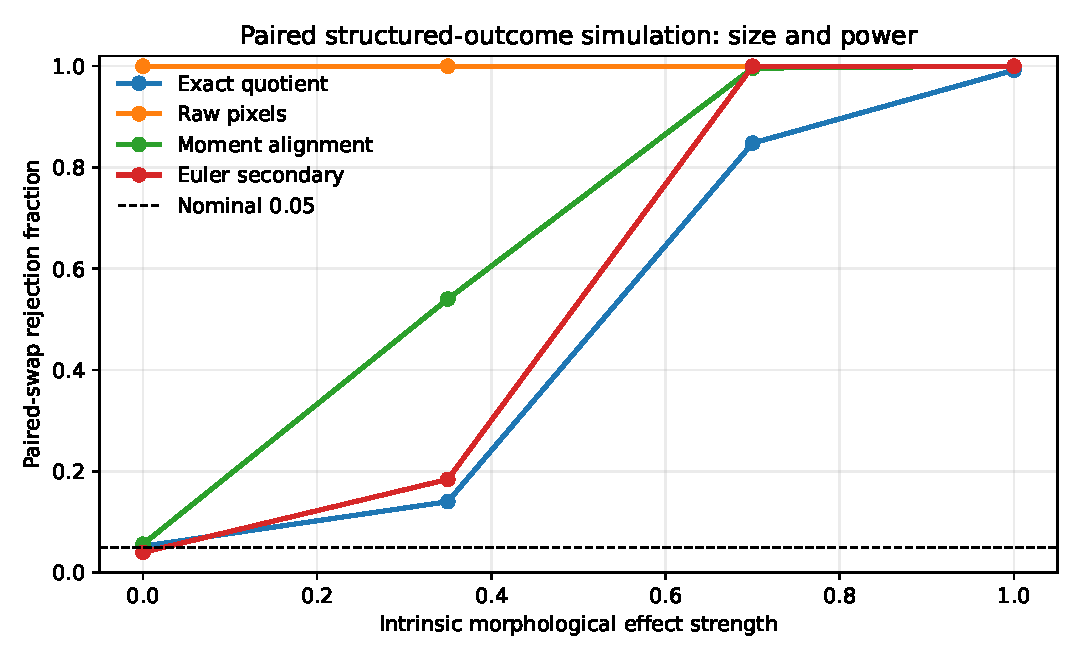
\includegraphics[width=.84\linewidth]{simulation_power.pdf}
\caption{Simulation rejection fractions. Finite-sample causal validity
	under informative acquisition pertains to the quotient and
	post-canonical Euler endpoints; the other methods are diagnostics.
	The exact quotient begins near the nominal 0.05 level and rises to
	\SimCanonicalPower, raw pixels remain at 1.0, and moment registration and the Euler
	endpoint begin near 0.05 and approach 1.0 as effect strength increases.
	\label{fig:simulation}}
\end{figure}

\FloatBarrier
\section{RxRx1 confirmation experiment}\label{sec:rxrx1}

\subsection{Units, selection and imposed acquisition}

The public RxRx1 release \citep{Recursion2023,Sypetkowski2023} contains 125,510 six-channel $512\times512$ images, with two nonoverlapping sites per well, 51 experimental batches, four cell types and 1,138 siRNAs, including 1,108 noncontrol perturbations. HUVEC contributes 24 batches. The well is the experimental unit; sites and pixels are components of one structured outcome, not independent replicates. The conditions are applied siRNA reagents, so the estimand is reagent-specific rather than automatically gene-specific.

HUVEC-01 through HUVEC-12 are used for discovery, HUVEC-13 through HUVEC-16
are reserved, and HUVEC-17 through HUVEC-24 supply
$\RxConfirmationBatches$ confirmation blocks. Selection uses public
128-dimensional embeddings from discovery rows only. The two site embeddings
are averaged within a well. Within each discovery batch and embedding
coordinate, noncontrol wells are median-centered and scaled by $1.4826$ times
the median absolute deviation; scales below $10^{-6}$ are replaced by 1.
Writing $E_{je}\in\R^{128}$ for the normalized embedding of condition $j$ in
experiment $e$, split the discovery batches into
$H_1=\{1,\ldots,6\}$ and $H_2=\{7,\ldots,12\}$ and set
\[
\begin{aligned}
\bar E_{jh}&=|H_h|^{-1}\sum_{e\in H_h}E_{je},&
V_{jh}&=|H_h|^{-1}\sum_{e\in H_h}\|E_{je}-\bar E_{jh}\|_2^2,\\
\delta_h(j,k)&=\bar E_{jh}-\bar E_{kh},&
R_h(j,k)&=\frac{\|\delta_h(j,k)\|_2^2}
{V_{jh}+V_{kh}+10^{-12}}.
\end{aligned}
\]
The discovery stability score is
\begin{equation}\label{eq:selection-score}
S(j,k)=
\min_{h\in\{1,2\}}R_h(j,k)
\max\left\{
\frac{\langle\delta_1(j,k),\delta_2(j,k)\rangle}
{\sqrt{(\|\delta_1(j,k)\|_2^2+10^{-12})
(\|\delta_2(j,k)\|_2^2+10^{-12})}},0\right\}.
\end{equation}
Eligibility requires one two-site well per condition in every discovery batch
and identical discovery plate signatures. Candidates are ordered by decreasing
$S(j,k)$, minimum half-SNR, direction cosine and mean half-SNR, with ascending
integer identifiers as the final tie-break; greedy matching gives
$\RxSelectedPairs$ disjoint pairs. The highest score defines the primary pair
and the other $\RxReplicationPairs$ pairs form the secondary family. Neither
confirmation metadata, confirmation embeddings nor confirmation images enter
the selector. The row split does not prove that the public embedding generator
was trained independently of every confirmation image, so complete algorithmic
independence remains an assumption.

The confirmation subset contains 160 wells, 320 sites and 1,920 single-channel
PNG files. Each site is converted to a six-channel finite-support lattice array
by $512$-to-$64$ Pillow BOX resampling, retention of 8-bit values and a
16-pixel zero border, giving a $96\times96$ storage canvas. The maximum imposed
translation is eight pixels per coordinate.

For the six-channel array $I_{ws}$ from well $w$ and site $s$, define
\[
m_{ws}=\operatorname{mean}(I_{ws}/255)
+0.25\,\operatorname{sd}(I_{ws}/255),
\qquad
\widetilde m=\operatorname{median}_{w,s}m_{ws}.
\]
For each of $\RxNuisanceSeeds$ published seeds, 20260731 through 20260750, the
UTF-8 string \texttt{seed|well\_id|}\allowbreak\texttt{site=s} is hashed to a
24-byte BLAKE2b digest, split into three little-endian unsigned 64-bit integers
$H_{0,ws},H_{1,ws},H_{2,ws}$. With treatment label
$a_w\in\{0,1\}$, put
\[
\begin{aligned}
b_{ws}&=\1\{m_{ws}>\widetilde m\},&
q_{ws}&=\lfloor1000003|m_{ws}|\rfloor,\\
r_{ws}&=(H_{0,ws}\bmod2+2a_w+b_{ws})\bmod4,&
d_w&=2a_w-1,\\
\Delta y_{ws}&=d_w\{1+(H_{1,ws}+q_{ws})\bmod8\},&
\Delta x_{ws}&=d_w\{1+(H_{2,ws}+7q_{ws}+b_{ws})\bmod8\}.
\end{aligned}
\]
All six channels at one site share the resulting quarter turn and translation,
while the two sites receive separate motions. The transformation is therefore
treatment- and outcome-dependent but remains inside the declared product
action. The realized parameters are logged for audit and excluded from every
representation and test routine. No interpolation is used, and the software
aborts if nonzero support is cropped. Seed 20260731 is the primary acquisition
realization used in Table~\ref{tab:primary}; the other 19 seeds assess exact
invariance and acquisition-only behavior.

\subsection{Confirmatory results}

The primary contrast is siRNA 384 (\RxTreatmentA) versus siRNA 747
(\RxTreatmentB). The completeness and same-plate gates \RxPlateAudit. The
discovery-only manifest has SHA-256 digest
{\scriptsize\texttt{\RxManifestHash}}.

\begin{table}[!htbp]
\caption{Primary RxRx1 pair under imposed lattice rigid motions for nuisance
seed 20260731. The quotient-pixel endpoint is the sole primary test; Euler is
an unadjusted secondary endpoint; moment registration is a diagnostic without
a proved maximal-invariance guarantee; raw pixels are an acquisition-sensitive
diagnostic.\label{tab:primary}}
\centering
\begin{tabular}{@{}lrr@{}}
\toprule
Representation & $\widehat{\MMD}_u^2$ & Paired-swap $p$\\
\midrule
Canonical quotient pixels & \RxCanonicalMMD & \RxCanonicalP\\
Finite directional Euler signature & \RxEulerMMD & \RxEulerP\\
Moment registration & \RxMomentMMD & \RxMomentP\\
Raw transformed pixels & \RxRawMMD & \RxRawP\\
\bottomrule
\end{tabular}
\end{table}

The prespecified paired-block bootstrap generated $\RxBootstrapReplicates$
resamples. Because sampling eight blocks with replacement duplicates
observations and changes the conventional observation-level U-statistic's
diagonal-exclusion structure, the resulting quantiles are not confidence
intervals or precision bounds. They are retained transparently as descriptive
quantiles of the resampled statistic.

\begin{table}[!htbp]
\caption{Prespecified bootstrap audit for the primary contrast. The final
column gives empirical 2.5th and 97.5th percentiles of the resampled
U-statistic, not confidence intervals.\label{tab:bootstrap-audit}}
\centering
\begin{tabular}{@{}lrr@{}}
\toprule
Representation & Original $\widehat{\MMD}_u^2$ & Resampled-statistic quantiles\\
\midrule
Canonical quotient pixels & \RxCanonicalMMD & \RxCanonicalMMDCI\\
Finite directional Euler signature & \RxEulerMMD & \RxEulerMMDCI\\
Moment registration & \RxMomentMMD & \RxMomentMMDCI\\
Raw transformed pixels & \RxRawMMD & \RxRawMMDCI\\
\bottomrule
\end{tabular}
\end{table}

\RxReplicationSummary\ Exact invariance held across all acquisition seeds:
maximum clean-versus-contaminated feature discrepancies were
\RxMaxQuotientFeatureError{} for canonical pixels and
\RxMaxEulerFeatureError{} for the Euler signature; the largest changes in the
quotient statistic and exact $p$-value were
\RxMaxQuotientStatisticError{} and \RxMaxQuotientPError. The algebraic audit
found \RxInvariantAuditFailures{} canonical-code failures among
\RxInvariantAuditTrials{} generated transformations. Twenty-nine pre-outcome
checks passed before the confirmatory analysis; the final expanded package
passed \SoftwareTestsPassed{} of \SoftwareTestsPassed{} tests.

\begin{table}[!htbp]
\caption{Canonical-quotient tests for the nine prespecified secondary contrasts. These contrasts are not biological replications of the primary contrast.\label{tab:secondary}}
\centering\scriptsize
\begin{tabular}{@{}clrrr@{}}
\toprule
Pair & Conditions & $\widehat{\MMD}_u^2$ & Swap $p$ & Holm $p$\\
\midrule
\RxReplicationRows
\bottomrule
\end{tabular}
\end{table}

For the acquisition-only control, the two clean well arrays in each
pair--block are averaged and rounded to 8-bit data. The identical prototype is
assigned to both conditions before the treatment-dependent hidden motion is
applied. This enforces the intrinsic sharp null while retaining informative
acquisition.

\begin{table}[t]
\caption{Acquisition-only sharp-null stress test over frozen pairs and nuisance seeds. Intervals are descriptive Clopper--Pearson summaries; pair--seed tests share biological blocks.\label{tab:sharpnull}}
\centering\small
\begin{tabular}{@{}lrrl@{}}
\toprule
Method & Tests & Rejections & Fraction (95\% interval)\\
\midrule
\RxAcquisitionNullRows
\bottomrule
\end{tabular}
\end{table}

For the off-action audit, every primary-pair site is first support-centered.
The two sites then receive opposite interpolated rotations $+\theta$ and
$-\theta$, two pixels are removed from all four support margins, or
within-support Gaussian noise with standard deviation 2 gray levels is added.
The label-free pooled bandwidth is recomputed separately for every
perturbation. If $Z_m^{(0)}$ and $Z_m^{(\delta)}$ are the baseline and
perturbed feature matrices for method $m$, the relative error is
\[
\varepsilon_m(\delta)=
\frac{\|Z_m^{(\delta)}-Z_m^{(0)}\|_F}
{\max\{\|Z_m^{(0)}\|_F,10^{-12}\}}.
\]
Thus Table~\ref{tab:approx} uses the support-centered exact-action baseline,
not the uncentered raw-pixel statistic in Table~\ref{tab:primary}.

\begin{table*}[t]
\caption{Approximate-action stress test for the primary pair. Feature error is relative to the exactly transformed baseline. These are empirical sensitivity results; Theorem~\ref{thm:stability} applies only when its Lipschitz assumptions are verified.\label{tab:approx}}
\centering\scriptsize
\begin{tabular}{@{}llrrr@{}}
\toprule
Perturbation & Method & Relative feature error & $|\Delta\widehat{\MMD}_u^2|$ & $|\Delta p|$\\
\midrule
\RxApproximateStressRows
\bottomrule
\end{tabular}
\end{table*}

\subsection{Post-outcome assignment sensitivity}

The bounded-odds analysis was specified after the primary outcome and result
had been accessed. It is therefore an exploratory robustness analysis and does
not alter the primary endpoint or exact paired-swap result. For each
$\Lambda$, the implementation enumerates all $\RxPermutationCount$
assignments and all $\RxPermutationCount$ vertices of the probability box in
\eqref{eq:sensitivity-model}.

\begin{table}[!htbp]
\caption{Post-outcome sensitivity of the primary quotient test to departure
from uniform paired assignment. The second column is the exact worst-case
upper-tail probability under~\eqref{eq:sensitivity-model}.
\label{tab:sensitivity}}
\centering
\begin{tabular}{@{}cc@{}}
\toprule
Sensitivity factor $\Lambda$ & Worst-case upper $p$\\
\midrule
\RxSensitivityRows
\bottomrule
\end{tabular}
\end{table}

At $\Lambda=1$, the envelope reproduces the complete paired-swap value
$\RxExtensionExactP$. The worst-case upper probability is 0.039171 at
$\Lambda=2$ and first reaches 0.05 at
$\Lambda=\RxSensitivityCritical$ (numerical upper probability
$\RxSensitivityCriticalP$). This quantifies departure from uniform allocation
within the independent bounded-odds model; it is not an estimate of a specific
unmeasured confounder.



\FloatBarrier
\section{Discussion}\label{sec:discussion}

Under unrestricted contamination, invariance is an observability requirement rather than a modeling preference. A noninvariant target can change while the observed law remains fixed; a maximal invariant captures the entire recoverable orbit. Causal identification then requires a separate design or exchangeability argument. The losslessness theorem adds a third distinction: even a maximal invariant may discard information about how probability is distributed within an orbit. Only a parameter-free conditional law, or a condition such as conditional Haar randomization that implies one, makes quotienting sufficient for the full statistical experiment.

The distinction between product and diagonal actions has practical consequences. Sitewise canonicalization is correct for the imposed RxRx1 mechanism because each site receives a separate motion. If a microscope applies one common transformation to all sites, a diagonal quotient should retain relative placement and orientation. Treating that problem as a product action would erase scientifically meaningful relational structure.

The approximate-contamination theorem links orbit error to quotient-law and MMD error, but it also clarifies the limits of the current stress test. Lexicographic canonicalization can be discontinuous. Large feature changes accompanied by stable $p$-values in Table~\ref{tab:approx} demonstrate test-level robustness for the frozen perturbations, not global representation stability. Establishing a Lipschitz quotient embedding on a scientifically relevant image class is a separate research problem.

A field-of-view crop is additionally a lossy observation operator. By
Theorem~\ref{thm:partial-observation}, an intrinsic target survives such an
operator only when it is constant on every fiber of the combined action and
crop map. The two-pixel experiment in Table~\ref{tab:approx} measures finite
sample sensitivity of this particular statistic; it does not establish
identifiability under arbitrary cropping.

The RxRx1 analysis is a controlled unknown-acquisition experiment on real biological images. Its content and batch structure are real; the transformation law is imposed and exactly audited. The causal conclusion is conditional on the reported within-plate assignment mechanism, well-defined reagent versions, no cross-well interference and swap-invariant retention. The primary result concerns a reagent-condition contrast, not automatically a gene-level mechanism. With eight pairs, exact enumeration is a strength, but the randomization distribution has coarse resolution.

The exploratory bounded-odds calculation addresses the most consequential
unverified part of that design premise. Its 0.05 crossing near
$\Lambda=\RxSensitivityCritical$ is meaningful only within the independent
product assignment model in~\eqref{eq:sensitivity-model}; it does not replace
documentation of the original randomization probabilities.

\section{Conclusion}\label{sec:conclusion}

Unknown transformations need not be estimated to conduct causal inference on the information that survives them. Under a measurable group action, orbit invariance is necessary and sufficient for uniform observability, and a maximal invariant contains every measurable observable target. Quotient reduction is statistically lossless only under the additional, exact boundary of a parameter-free conditional law given the quotient; conditional Haar contamination is one useful special case. Correct specification of product or diagonal actions determines whether relative component information is preserved. The lattice construction, characteristic quotient kernel and complete paired randomization test turn these distinctions into an auditable workflow for structured outcomes under informative acquisition.

\section*{Data availability}
The analysis uses the public RxRx1 dataset subject to its stated licence. The
companion reproducibility archive contains the frozen selection and integrity
manifests, retrieval and verification scripts, analysed code, machine-readable
results and manuscript-building inputs. The licensed RxRx1 image files are not
redistributed; the archive reacquires the frozen subset from the official
release and verifies every file before analysis.

\section*{Reproducibility statement}
The analysis software downloads the frozen RxRx1 subset, verifies file and
manifest hashes, constructs all representations, enumerates the complete
assignment distribution, performs multiplicity adjustment and sensitivity
analyses, executes unit tests and writes the numerical outputs consumed by the
manuscript. The legacy fingerprint
\texttt{source-\allowbreak e9f042c387cf} covers the core files used by the
original results builder. For the present release, the companion archive also
contains a path-by-path SHA-256 manifest of the complete analysed Python source,
scripts, tests and dependency specification; the SHA-256 digest of that manifest
is \texttt{\AnalysisSourceManifestHash}. A current-source rerun audit records
the commands, environment, file hashes and comparisons with the frozen outputs.

\section*{Author contributions}
Usef Faghihi and Amir Saki contributed equally to the conception,
methodology, theoretical development, analysis, interpretation of
results and preparation of the manuscript. Both authors reviewed and
approved the final manuscript.


\section*{Funding}
This research received no specific grant from any funding agency in
the public, commercial or not-for-profit sectors.
\section*{Acknowledgements and use of AI-assisted tools}
During manuscript preparation, the authors used OpenAI Codex for language editing, theorem-structure review and LaTeX reformatting. The authors are responsible for verifying all mathematical statements, empirical results, citations and final wording.

\appendix
\renewcommand{\thesection}{\Alph{section}}
\renewcommand{\theHsection}{appendix.\Alph{section}}
\section{Proof and measurability details}\label{sec:appendix}

\subsection{Proof of Theorem~\ref{thm:factorization}}


\begin{proof}
	Fix an arbitrary Borel set \(B\subseteq\calT\), and write
	\[
	E:=h^{-1}(B).
	\]
	Since \(h\) is Borel, both \(E\) and \(\calY\setminus E\) are Borel subsets of
	\(\calY\). We first verify explicitly that \(E\) is saturated with respect to
	the fibres of \(M\), that is,
	\[
	M^{-1}\{M(E)\}=E.
	\]
	The inclusion \(E\subseteq M^{-1}\{M(E)\}\) is immediate. Conversely, suppose
	that \(y\in M^{-1}\{M(E)\}\). Then there exists \(z\in E\) such that
	\(M(y)=M(z)\). By maximality of \(M\), there is some \(g\in G\) for which
	\(y=g\cdot z\). Invariance of \(h\) therefore gives
	\[
	h(y)=h(g\cdot z)=h(z)\in B,
	\]
	and hence \(y\in E\). This proves the asserted saturation. Notice that this
	statement concerns the particular set \(E=h^{-1}(B)\): it says that every
	fibre of \(M\) is either entirely contained in \(E\) or entirely contained in
	its complement; it does not assert that the fibres of \(M\) are singletons.
	
	We next claim that
	\[
	M(E)\cap M(\calY\setminus E)=\varnothing.
	\]
	Indeed, if \(s\) belonged to this intersection, there would exist
	\(y\in E\) and \(z\in\calY\setminus E\) such that
	\[
	M(y)=s=M(z).
	\]
	Maximality of \(M\) would then place \(y\) and \(z\) in the same \(G\)-orbit,
	so invariance of \(h\) would imply \(h(y)=h(z)\). This is impossible because
	\(h(y)\in B\), whereas \(h(z)\notin B\).
	
	Because \(\calY\) and \(\calS\) are standard Borel spaces, and \(M\) is
	Borel, the images \(M(E)\) and \(M(\calY\setminus E)\) are analytic subsets
	of \(\calS\). They need not themselves be Borel, which is why a separation
	argument is required. By Lusin's separation theorem, there exists a Borel
	set \(D_B\subseteq\calS\) satisfying
	\[
	M(E)\subseteq D_B
	\qquad\text{and}\qquad
	M(\calY\setminus E)\subseteq\calS\setminus D_B.
	\]
	We now show that
	\[
	E=M^{-1}(D_B).
	\]
	If \(y\in E\), then \(M(y)\in M(E)\subseteq D_B\), and hence
	\(y\in M^{-1}(D_B)\). If \(y\notin E\), then
	\(M(y)\in M(\calY\setminus E)\subseteq\calS\setminus D_B\), and hence
	\(y\notin M^{-1}(D_B)\). The two inclusions therefore follow, and
	\[
	h^{-1}(B)=E=M^{-1}(D_B)\in\sigma(M).
	\]
	
	Since \(B\subseteq\calT\) was an arbitrary Borel set, \(h\) is
	\(\sigma(M)\)-measurable. The measurable factorization lemma, applicable
	because \(\calT\) is a standard Borel space, therefore yields a Borel map
	\[
	\bar h:\calS\longrightarrow\calT
	\]
	such that
	\[
	h=\bar h\circ M.
	\]
	
	It remains to establish the stated uniqueness. Suppose that
	\(\bar h_1,\bar h_2:\calS\to\calT\) are two Borel maps satisfying
	\[
	h=\bar h_1\circ M=\bar h_2\circ M.
	\]
	For any \(s\in M(\calY)\), choose \(y\in\calY\) with \(M(y)=s\). Then
	\[
	\bar h_1(s)
	=\bar h_1\{M(y)\}
	=h(y)
	=\bar h_2\{M(y)\}
	=\bar h_2(s).
	\]
	Thus \(\bar h_1=\bar h_2\) on \(M(\calY)\). No uniqueness is claimed outside
	\(M(\calY)\), since values of a factor map there do not affect its
	composition with \(M\).
\end{proof}


\subsection{Existence constructions for maximal invariants}

\begin{proposition}[Orbit code for a compact action]
\label{prop:compact-orbit-code}
Let $G$ be a compact metrizable group acting continuously on a Polish space
$\calY$. Let $\calK(\calY)$ be the hyperspace of nonempty compact subsets of
$\calY$, equipped with its Vietoris Borel structure. Then
\[
M_{\rm orb}(y)=G\cdot y
\]
is a Borel maximal invariant taking values in the standard Borel space
$\calK(\calY)$.
\end{proposition}

\begin{proof}
The orbit is compact because it is the continuous image of compact $G$. For
an open set $U\subseteq\calY$,
\[
\{y:M_{\rm orb}(y)\cap U\ne\varnothing\}
=\bigcup_{g\in G}g^{-1}U,
\]
which is open. Also,
\[
\{y:M_{\rm orb}(y)\subseteq U\}
=\calY\setminus\bigcup_{g\in G}g^{-1}(\calY\setminus U).
\]
To see directly that this second set is open, fix $y$ with $G\cdot y\subset U$.
For every $g\in G$, joint continuity gives neighborhoods $N_g$ of $g$ and
$V_g$ of $y$ with $N_g\cdot V_g\subset U$. Compactness supplies
$g_1,\ldots,g_r$ with $G=\bigcup_iN_{g_i}$. Then
$V=\bigcap_iV_{g_i}$ is a neighborhood of $y$ satisfying $G\cdot V\subset U$.
These two classes generate the Vietoris topology, so $M_{\rm orb}$ is
continuous and therefore Borel. Finally,
$M_{\rm orb}(y)=M_{\rm orb}(z)$ exactly when $z\in G\cdot y$, proving
maximality.
\end{proof}

This result is orbit-valued; it does not by itself construct a
finite-dimensional representative. It also does not cover a noncompact group
such as $\operatorname{SE}(2)$. The lattice construction in
Section~\ref{sec:lattice} instead supplies an explicit cross-section for its
noncompact integer-translation component.

\begin{proposition}[Canonical code for a finite group]
\label{prop:finite-canonical}
Let a finite group $H=\{h_1,\ldots,h_m\}$ act by Borel maps on a standard
Borel space $\calY$, and let $\nu:\calY\to[0,1]$ be a Borel injection. Define
\[
j^\star(y)=\min\argmin_{1\le j\le m}\nu(h_j\cdot y),
\qquad c_H(y)=h_{j^\star(y)}\cdot y.
\]
Then $c_H$ is a Borel maximal invariant for the $H$-action.
\end{proposition}

\begin{proof}
Put $f_j(y)=\nu(h_j\cdot y)$. Each $f_j$ is Borel, and
\[
\{y:j^\star(y)=j\}
=
\bigcap_{k<j}\{y:f_j(y)<f_k(y)\}
\cap
\bigcap_{k>j}\{y:f_j(y)\le f_k(y)\}.
\]
Thus $j^\star$ and $c_H$ are Borel. Let
$\calO_y=\{h\cdot y:h\in H\}$ be the finite set of distinct orbit points.
Injectivity of $\nu$ gives a unique least point $u_y$ in $\calO_y$ by its
$\nu$-value. Multiple minimizing indices can occur only when they represent
that same point, as under a nontrivial stabilizer, so $c_H(y)=u_y$. If
$z=h\cdot y$, the two orbits coincide and $c_H(z)=c_H(y)$. Conversely, if
$c_H(z)=c_H(y)$, the two orbits intersect and hence coincide. Thus $z$ and
$y$ are in the same $H$-orbit.
\end{proof}

The lattice construction combines an explicit cross-section for noncompact
translations with this finite residual minimization.

\subsection{Measurability of the Haar orbit kernel}

For compact second-countable $G$, a jointly Borel action and measurable section make $m\mapsto K_m(B)$ in~\eqref{eq:haar-kernel} measurable for every Borel $B$ by integration of the jointly measurable indicator $(g,m)\mapsto\1\{g\cdot s(m)\in B\}$. Stabilizers may change the map from $G$ onto an orbit but do not change the pushforward orbit measure.

\begin{thebibliography}{99}

\bibitem{Bhattacharjee2025}
Bhattacharjee, S., Li, B., Wu, X. and Xue, L. (2025) Doubly robust estimation of causal effects for random object outcomes with continuous treatments. \emph{arXiv:2506.22754}.

\bibitem{Blackwell1953}
Blackwell, D. (1953) Equivalent comparisons of experiments. \emph{Ann. Math. Statist.}, 24, 265--272.

\bibitem{ClopperPearson1934}
Clopper, C. J. and Pearson, E. S. (1934) The use of confidence or fiducial limits illustrated in the case of the binomial. \emph{Biometrika}, 26, 404--413.

\bibitem{Curry2022}
Curry, J., Mukherjee, S. and Turner, K. (2022) How many directions determine a shape and other sufficiency results for two topological transforms. \emph{Trans. Amer. Math. Soc. Ser. B}, 9, 1006--1043.

\bibitem{Eaton1989}
Eaton, M. L. (1989) \emph{Group Invariance Applications in Statistics}. Institute of Mathematical Statistics, Hayward, CA.

\bibitem{Fisher1935}
Fisher, R. A. (1935) \emph{The Design of Experiments}. Oliver and Boyd, Edinburgh.

\bibitem{Gretton2012}
Gretton, A., Borgwardt, K. M., Rasch, M. J., Sch\"olkopf, B. and Smola, A. (2012) A kernel two-sample test. \emph{J. Mach. Learn. Res.}, 13, 723--773.

\bibitem{Holm1979}
Holm, S. (1979) A simple sequentially rejective multiple test procedure. \emph{Scand. J. Stat.}, 6, 65--70.

\bibitem{Kallenberg2021}
Kallenberg, O. (2021) \emph{Foundations of Modern Probability}, 3rd edn. Springer, Cham.

\bibitem{Kechris1995}
Kechris, A. S. (1995) \emph{Classical Descriptive Set Theory}. Springer, New York.

\bibitem{Kurisu2024}
Kurisu, D., Zhou, Y., Otsu, T. and M\"uller, H.-G. (2024) Geodesic causal inference. \emph{arXiv:2406.19604}.

\bibitem{LeCam1986}
Le Cam, L. (1986) \emph{Asymptotic Methods in Statistical Decision Theory}. Springer, New York.

\bibitem{LehmannRomano2005}
Lehmann, E. L. and Romano, J. P. (2005) \emph{Testing Statistical Hypotheses}, 3rd edn. Springer, New York.

\bibitem{Otsu1979}
Otsu, N. (1979) A threshold selection method from gray-level histograms. \emph{IEEE Trans. Syst. Man Cybern.}, 9, 62--66.

\bibitem{Raykov2025}
Raykov, Y. P., Luo, H., Strait, J. D. and KhudaBukhsh, W. R. (2025) Kernel-based estimators for functional causal effects. \emph{arXiv:2503.05024}.

\bibitem{Recursion2023}
[dataset] Recursion (2023) RxRx1: an image set for cellular morphological variation across many biological perturbations. \url{https://www.rxrx.ai/rxrx1}.

\bibitem{Robins1986}
Robins, J. M. (1986) A new approach to causal inference in mortality studies with a sustained exposure period. \emph{Math. Modelling}, 7, 1393--1512.

\bibitem{RosenbaumRubin1983}
Rosenbaum, P. R. and Rubin, D. B. (1983) The central role of the propensity score in observational studies for causal effects. \emph{Biometrika}, 70, 41--55.

\bibitem{Rubin1974}
Rubin, D. B. (1974) Estimating causal effects of treatments in randomized and nonrandomized studies. \emph{J. Educ. Psychol.}, 66, 688--701.

\bibitem{Shin2024}
Shin, H.-Y., Kim, K., Lee, K. and Oh, H.-S. (2024) Absolute average and median treatment effects as causal estimands on metric spaces. \emph{arXiv:2407.03726}.

\bibitem{Sriperumbudur2010}
Sriperumbudur, B. K., Gretton, A., Fukumizu, K., Sch\"olkopf, B. and Lanckriet, G. R. G. (2010) Hilbert space embeddings and metrics on probability measures. \emph{J. Mach. Learn. Res.}, 11, 1517--1561.

\bibitem{Sypetkowski2023}
Sypetkowski, M. et al. (2023) RxRx1: a dataset for evaluating experimental
batch correction methods. In \emph{2023 IEEE/CVF Conference on Computer
Vision and Pattern Recognition Workshops (CVPRW)}.
doi:\href{https://doi.org/10.1109/CVPRW59228.2023.00451}{10.1109/CVPRW59228.2023.00451}.

\bibitem{Torgersen1991}
Torgersen, E. (1991) \emph{Comparison of Statistical Experiments}. Cambridge University Press, Cambridge.

\bibitem{Turner2014}
Turner, K., Mukherjee, S. and Boyer, D. M. (2014) Persistent homology transform for modeling shapes and surfaces. \emph{Information and Inference}, 3, 310--344.

\bibitem{Wijsman1990}
Wijsman, R. A. (1990) \emph{Invariant Measures on Groups and Their Use in Statistics}. Institute of Mathematical Statistics, Hayward, CA.

\end{thebibliography}

\section*{Figure caption list}
\noindent Figure~\ref{fig:simulation}. Simulation rejection fractions across intrinsic effect strengths; causal validity under informative acquisition pertains to invariant endpoints.

\section*{Table caption list}
\noindent Table~\ref{tab:simulation}. Simulation rejection fractions.\\
Table~\ref{tab:primary}. Primary RxRx1 contrast.\\
Table~\ref{tab:bootstrap-audit}. Prespecified bootstrap audit.\\
Table~\ref{tab:secondary}. Prespecified secondary contrasts.\\
Table~\ref{tab:sharpnull}. Acquisition-only sharp-null stress test.\\
Table~\ref{tab:approx}. Approximate-action stress test.\\
Table~\ref{tab:sensitivity}. Post-outcome bounded-odds sensitivity analysis.

\end{document}
